\documentclass[11pt,a4paper]{article}
\usepackage[utf8]{inputenc}
\usepackage{amsmath}
\usepackage{amsfonts}
\usepackage{amssymb}
\usepackage{booktabs}
\usepackage{geometry}
\usepackage{tabularx}
\usepackage{tikz}
\usepackage{caption}
\usepackage{fancyhdr}
\usepackage{float} 
\usepackage[style=numeric,backend=biber]{biblatex}

% Load bibliography file
\addbibresource{references.bib}

\usetikzlibrary{decorations.pathmorphing, arrows.meta, positioning}
\geometry{margin=1in, headheight=14pt}

% Configure Fancy Headers & Footers
\pagestyle{fancy}
\fancyhf{}
\fancyhead[L]{\small\scshape The Grand Unified Monograph}
\fancyhead[R]{\small\thepage}
\fancyfoot[C]{\small Geometry as the Fabric of Force}
\renewcommand{\headrulewidth}{0.4pt}
\renewcommand{\footrulewidth}{0.0pt}

\begin{document}

% --- PROFESSIONAL TEXTBOOK TITLE PAGE ---
\begin{titlepage}
    \pagestyle{empty} 
    \centering
    \vspace*{3cm}
    
    {\Huge\bfseries The Grand Unified Monograph \par}
    \vspace{0.8cm}
    {\Large\scshape Geometry as the Fabric of Force \par}
    
    \vspace{2cm}
    {\large\bfseries Advanced Mathematical Reference Manual \par}
    
    \vfill
    
    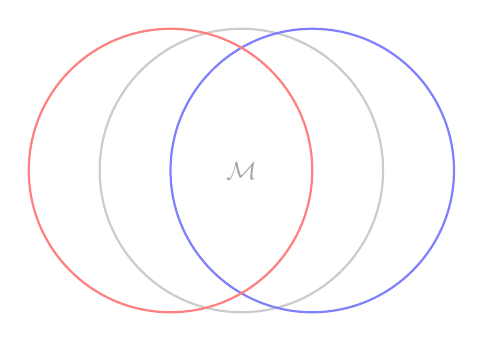
\begin{tikzpicture}[scale=1.5]
        \draw[thick, gray!40] (0,0) circle (1.2);
        \draw[thick, blue!50] (0.6,0) circle (1.2);
        \draw[thick, red!50] (-0.6,0) circle (1.2);
        \node[gray!70] at (0,0) {\small $\mathcal{M}$};
    \end{tikzpicture}
    
    \vfill
    
    {\large September 22, 2026 \par}
    \vspace*{2cm}
\end{titlepage}
\newpage

\begin{abstract}
\noindent This monograph establishes a continuous mathematical framework linking classical planetary orbits, non-Abelian gauge fields, pseudo-Riemannian spacetime geometry, and non-perturbative quantum gravitational horizons into a single unified geometric formalism.
\end{abstract}

\tableofcontents
\newpage

\section*{Summary Matrix}
\addcontentsline{toc}{section}{Summary Matrix}
\begin{table}[H] 
\centering
\def\arraystretch{0.95} % Compressed from 1.1 to squeeze vertical space
\fontsize{8.5pt}{10pt}\selectfont % Adjusted slightly down from 9pt
\begin{tabularx}{\textwidth}{l l l X}
\toprule
\textbf{Physics Domain} & \textbf{Governing Equation} & \textbf{Geometric Operator} & \textbf{Core Physical Reality} \\ \midrule
Classical Mechanics & $T^2 = \left(\frac{4\pi^2}{GM}\right)r^3$ & Radius Vector ($\mathbf{r}$) & Conservation of Angular Momentum \\ \addlinespace[2pt]
Electrostatics & $\mathbf{F} = \frac{1}{4\pi\varepsilon_0}\frac{q_1 q_2}{r^2}\mathbf{\hat{r}}$ & Radial Unit Vector ($\mathbf{\hat{r}}$) & 3D space surface area scaling ($4\pi r^2$) \\ \addlinespace[2pt]
Field Dynamics & $\partial_{\nu} T^{\mu\nu} = -F^{\mu\nu} J_{\nu}$ & Stress Tensor ($T^{\mu\nu}$) & Energy-momentum flux embedding \\ \addlinespace[2pt]
Electrodynamics & $d\star F = -\mu_0 J$ & Exterior Derivative ($d, \star$) & Interwoven spacetime field fluxes \\ \addlinespace[2pt]
Gauge Gravity & $S_P = \frac{1}{64\pi G}\int \epsilon_{abcd}e^a\wedge e^b\wedge R^{cd}$ & Tetrad \& Spin Conn. ($e^a, \omega^a_{\ b}$) & Metric-independent frame coordinates \\ \addlinespace[2pt]
QFT in Curved Space & $\hat{b}_j = \sum_i (\alpha_{ji}\hat{a}_i - \beta_{ji}^*\hat{a}_i^{\dagger})$ & Bogoliubov Maps ($\alpha, \beta$) & Horizon-induced mode mixing bath \\ \addlinespace[2pt]
General Relativity & $G_{\mu\nu} + \Lambda g_{\mu\nu} = \frac{8\pi G}{c^4} T_{\mu\nu}$ & Einstein Tensor ($G_{\mu\nu}$) & Spacetime curvature dictated by matter \\ \addlinespace[2pt]
Quantum Foundations & $\hat{H}_{\text{Wheeler-DeWitt}}|\Psi\rangle = 0$ & Super-Hamiltonian ($\hat{H}$) & Timeless metric state configuration space \\ \addlinespace[2pt]
Topological Fields & $S_{\text{CS}} = \frac{k}{4\pi} \int \text{Tr}(A \wedge dA - \frac{2}{3}i A^3)$ & Chern-Simons Form ($\wedge$) & Global boundary invariants and anomalies \\ \addlinespace[2pt]
Supersymmetry & $\{Q_{\alpha}, \bar{Q}_{\dot{\beta}}\} = 2\sigma^{\mu}_{\alpha\dot{\beta}} P_{\mu}$ & Supercharges ($Q, \bar{Q}$) & Graded Lie algebraic transformations \\ \addlinespace[2pt]
String Theory & $S_P = -\frac{T}{2} \int d^2\sigma \sqrt{- \gamma}\gamma^{\alpha\beta}\partial_{\alpha} X \cdot \partial_{\beta} X$ & Polyakov Action ($\gamma^{\alpha\beta}$) & 2D worldsheet metric embeddings \\ \addlinespace[2pt]
Holography & $S_A = \frac{\text{Area}(\gamma_A)}{4G_N}$ & Minimal Surface ($\gamma_A$) & Bulk minimal area mapping entanglement \\ \addlinespace[2pt]
Statistical Mechanics & $Z = \sum_i e^{-\beta E_i}$ & Boltzmann Factor ($\beta$) & Discrete microstate phase space scaling \\ \addlinespace[2pt]
Standard Model & $\mathcal{L}_{\text{SM}} = \bar{\psi}_i i\gamma^{\mu} D_{\mu} \psi_i + |D_{\mu}\phi|^2 - V(\phi)$ & Covariant Derivative ($D_{\mu}$) & Spontaneous local gauge symmetry breaking \\ \addlinespace[2pt]
Early Inflation & $\mathcal{P}_{\mathcal{R}}(k) = \frac{H^2}{2\pi \dot{\phi}}\biggr\vert_{k=aH}$ & Inflaton Fluctuations ($\delta\phi$) & Quantum modes frozen to cosmic structure \\ \addlinespace[2pt]
Cosmology & $(\frac{\dot{a}}{a})^2 = \frac{8\pi G}{3}\rho - \frac{kc^2}{a^2} + \frac{\Lambda c^2}{3}$ & Cosmic Conformal Scaling ($a$) & Isotropic expansion of global universe \\ \bottomrule
\end{tabularx}
\caption{Comprehensive structural matrix mapping physical regimes to geometric frameworks.}
\end{table}

\newpage


\section*{Section 0: Mathematical Appendix \& Gauge Foundations}
\addcontentsline{toc}{section}{Section 0: Mathematical Appendix \& Gauge Foundations}
To maintain rigorous consistency across classical, relativistic, and quantum fields, our notation utilizes coordinate-free differential forms and Lie algebraic generators.

\subsection*{0.1 Exterior Calculus on Manifolds}
Let $M$ be a smooth, oriented pseudo-Riemannian manifold of dimension $n$ equipped with a metric $g$. A differential $p$-form $\omega \in \Omega^p(M)$ is a totally antisymmetric tensor of type $(0,p)$. The exterior derivative $d: \Omega^p(M) \rightarrow \Omega^{p+1}(M)$ is a nilpotent operator ($d^2 = 0$). The wedge product $\wedge: \Omega^p(M) \times \Omega^q(M) \rightarrow \Omega^{p+q}(M)$ obeys:
\begin{equation}
    \alpha \wedge \beta = (-1)^{pq} \beta \wedge \alpha
\end{equation}
We formally introduce the Hodge star operator $\star: \Omega^p(M) \rightarrow \Omega^{n-p}(M)$, which maps any $p$-form to its unique $(n-p)$-form dual. Given the natural volume form $\eta$, the Hodge dual is uniquely defined via the inner product relationship for any two $p$-forms $\alpha$ and $\beta$:
\begin{equation}
    \alpha \wedge \star \beta = g(\alpha, \beta) \, \eta
\end{equation}
For our $n=4$ Lorentzian spacetime fabric, applying the operator twice to a $p$-form yields $\star \star \omega = (-1)^{p(4-p)+1} \omega$, dictating the crucial relative negative signs found in our physical field variations.

\subsection*{0.2 Non-Abelian Field Tensors \& Algebra Structural Identities}
For a principal fiber bundle with a compact Lie gauge group $G$, the connection 1-form is $A = A_{\mu}^a T^a dx^{\mu}$, where $T^a$ are hermitian generators satisfying $[T^a, T^b] = i f^{abc} T^c$. The curvature 2-form (field strength tensor) is:
\begin{equation}
    F = dA - i g A \wedge A \implies F_{\mu\nu}^a = \partial_{\mu} A_{\nu}^a - \partial_{\nu} A_{\mu}^a + g f^{abc} A_{\mu}^b A_{\nu}^c
\end{equation}
Enforcing the algebraic Jacobi Identity $[T^a,[T^b,T^c]] + [T^b,[T^c,T^a]] + [T^c,[T^a,T^b]] = 0$ dictates a structural constraint on the structure constants $f^{abc}$:
\begin{equation}
    f^{ade}f^{bcd} + f^{bde}f^{cad} + f^{cde}f^{abd} = 0
\end{equation}
The gauge covariant derivative preserving local physical mapping transformations under a specified field representation is formulated as:
\begin{equation}
    D_{\mu} = \partial_{\mu} - i g A_{\mu}^a T^a
\end{equation}

\section{Classical Mechanics \& Gravitational Fields}
The real physical trajectory extremizes the Action path integral functional $S$:
\begin{equation}
    \delta S = \delta \int_{t_1}^{t_2} L(q, \dot{q}, t) \, dt = 0
\end{equation}
Planets trace out elliptical orbits with the central mass located at one focus. The area conservation rate is directly proportional to angular momentum $L$:
\begin{equation}
    \frac{dA}{dt} = \frac{L}{2m} = \text{constant}, \quad T^2 = \left(\frac{4\pi^2}{GM}\right)r^3
\end{equation}
Equating centripetal force to Newtonian gravitational force yields:
\begin{equation}
    \frac{mv^2}{r} = \frac{GMm}{r^2} \implies v^2 = \frac{GM}{r}
\end{equation}
Substituting the orbital boundary velocity circumference constraint $v = \frac{2\pi r}{T}$:
\begin{equation}
    \left(\frac{2\pi r}{T}\right)^2 = \frac{GM}{r} \implies \frac{4\pi^2 r^2}{T^2} = \frac{GM}{r} \implies T^2 = \left(\frac{4\pi^2}{GM}\right)r^3
\end{equation}

\section{Electrostatics \& Geometric Derivations}
\begin{equation}
    \mathbf{F} = \frac{1}{4\pi\varepsilon_0}\frac{q_1 q_2}{r^2}\mathbf{\hat{r}}, \quad \oint_S \mathbf{E} \cdot d\mathbf{A} = \frac{Q_{\text{encl}}}{\varepsilon_0}
\end{equation}
Constructing a spherical closed manifold $S$ of radius $r$ centered on isolated charge $q$:
\begin{equation}
    \oint_S \mathbf{E} \cdot d\mathbf{A} = E \oint_S dA = E(4\pi r^2) = \frac{q}{\varepsilon_0} \implies E = \frac{1}{4\pi\varepsilon_0}\frac{q}{r^2}
\end{equation}
The force evaluating expression $\mathbf{F} = q_2\mathbf{E}$ proves that the inverse-square decay of electrostatics is a direct mathematical consequence of 3D spatial boundaries scaling as $4\pi r^2$.

\section{Classical Field Theory and the Stress-Energy Tensor}
To demonstrate how the classical Maxwell system naturally demands a four-dimensional spacetime architecture, we map its energy, momentum, and stress distributions into a unified symmetric tensor of rank two. We define the electromagnetic stress-energy tensor $T^{\mu\nu}$ by varying the Maxwell action with respect to the background spacetime metric $g^{\mu\nu}$:
\begin{equation}
    T^{\mu\nu} = \frac{1}{\mu_0} \left( F^{\mu\alpha} F^{\nu}_{\ \alpha} - \frac{1}{4} g^{\mu\nu} F_{\alpha\beta} F^{\alpha\beta} \right)
\end{equation}
By computing the spacetime divergence of this tensor, we invoke the inhomogeneous Maxwell field equations ($\partial_{\alpha} F^{\alpha\mu} = -\mu_0 J^{\mu}$) alongside the geometric Bianchi identity ($F_{[\alpha\beta,\gamma]} = 0$). This directly yields the conservation law:
\begin{equation}
\partial_{\nu} T^{\mu\nu} = -F^{\mu\nu} J_{\nu}
\end{equation}
where the right-hand side represents the exact coordinate components of the Lorentz force density. This framework proves that electromagnetic fields do not merely inhabit space; they actively store energy-momentum density, serving as a direct geometric source capable of warping the spacetime fabric via the Einstein field equations.
\section{The Gauge View of Gravity: Tetrads and Palatini Formalism}
To couple fermionic fields (Clifford spinors $\psi$) to a curved pseudo-Riemannian manifold $(\mathcal{M}, g)$, the coordinate tangent space maps directly to a flat, internal Minkowski space $\eta_{ab} = \text{diag}(-1,1,1,1)$:
\begin{equation}
g_{\mu\nu} = e^a_{\mu} e^b_{\nu} \eta_{ab}, \quad \text{and} \quad \eta_{ab} = e_a^{\mu} e_b^{\nu} g_{\mu\nu}
\end{equation}
To preserve local Lorentz invariance $\psi \mapsto \Lambda(x)\psi$, we define a gauge connection 1-form $\omega^a_{\ b} = \omega^a_{\ b\mu} dx^{\mu}$ valued in the $\mathfrak{so}(1,3)$ Lie algebra. The directional covariant derivative acting on a Dirac spinor field is structured as:
\begin{equation}
D_{\mu} \psi = \left( \partial_{\mu} - \frac{i}{4} \omega_{\mu ab} \sigma^{ab} \right) \psi
\end{equation}
where $\sigma^{ab} = \frac{i}{2}[\gamma^a, \gamma^b]$ are the local generators of the Clifford algebra obeying ${\gamma^a, \gamma^b} = 2\eta^{ab}$. The gauge curvature 2-form $R^a_{\ b} = \frac{1}{2} R^a_{\ b\mu\nu} dx^{\mu} \wedge dx^{\nu}$ is governed by the structural Cartan identity:
\begin{equation}
R^a_{\ b} = d\omega^a_{\ b} + \omega^a_{\ c} \wedge \omega^c_{\ b}
\end{equation}
The Palatini approach is a first-order formalism where the tetrad $e^a$ and the spin connection $\omega^a_{\ b}$ are treated as completely independent dynamical variables:
\begin{equation}
S_P[e, \omega] = \frac{1}{64\pi G} \int_{\mathcal{M}} \epsilon_{abcd} e^a \wedge e^b \wedge R^{cd}(\omega)
\end{equation}
Extremizing the action path yields the structural constraint equation:
\begin{equation}
D(e^a \wedge e^b) = 0 \implies \mathcal{T}^a \wedge e^b - e^a \wedge \mathcal{T}^b = 0
\end{equation}
where $\mathcal{T}^a = de^a + \omega^a_{\ b} \wedge e^b$ defines the Cartan Torsion 2-form. In a vacuum, this dictates that spacetime is torsion-free ($\mathcal{T}^a = 0$). Varying with respect to the frame field $e^a$ generates the vacuum Einstein Field Equations:
\begin{equation}
\epsilon_{abcd} e^b \wedge R^{cd}(\omega) = 0 \implies R_{\mu\nu} - \frac{1}{2}g_{\mu\nu}R = 0
\end{equation}
\section{The Full Classical Maxwell System: A Variational Approach}
\begin{equation}
F = dA \implies dF = d(dA) = 0
\end{equation}
To maintain strict SI unit consistency, we explicitly include the vacuum permeability $\mu_0$ within the interaction term. We define the electromagnetic action functional $S[A]$ in terms of the field strength 2-form $F$, its Hodge dual $\star F$, and the source 1-form $J$ representing the charge-current density:
\begin{equation}
S[A] = -\frac{1}{2} \int_{\mathcal{M}} F \wedge \star F - \mu_0 \int_{\mathcal{M}} A \wedge J
\end{equation}
\subsection*{Variational Derivation of Field Equations}
We now apply a dynamic variation to the potential field, transforming $A \to A + \delta A$, where the variation $\delta A$ vanishes smoothly at the spatial and temporal boundaries of the manifold ($\partial\mathcal{M} = 0$). By taking the variation of the action $\delta S = 0$:
\begin{equation}
\delta S = -\frac{1}{2} \int_{\mathcal{M}} \left( \delta F \wedge \star F + F \wedge \delta(\star F) \right) - \mu_0 \int_{\mathcal{M}} \delta A \wedge J
\end{equation}
Utilizing the symmetry property of the wedge product and the Hodge star operator for differential forms on a Lorentzian manifold, $\delta F \wedge \star F = F \wedge \star \delta F$, the kinetic variation simplifies to:
\begin{equation}
\delta S = - \int_{\mathcal{M}} d(\delta A) \wedge \star F - \mu_0 \int_{\mathcal{M}} \delta A \wedge J
\end{equation}
To isolate the field variation $\delta A$, we apply the graded Leibniz rule for exterior derivatives, noting that $\delta A$ is a 1-form:
\begin{equation}
d(\delta A \wedge \star F) = d(\delta A) \wedge \star F - \delta A \wedge d\star F
\end{equation}
Solving for the kinetic term $d(\delta A) \wedge \star F$ and distributing the leading negative sign across both resulting elements yields:
\begin{equation}
\delta S = - \int_{\mathcal{M}} d(\delta A \wedge \star F) - \int_{\mathcal{M}} \delta A \wedge d\star F - \mu_0 \int_{\mathcal{M}} \delta A \wedge J
\end{equation}
By applying Stokes' Theorem, the boundary term vanishes completely. The remaining terms are grouped inside the manifold integral:
\begin{equation}
\delta S = -\int_{\mathcal{M}} \delta A \wedge \left( d\star F + \mu_0 J \right)
\end{equation}
For the action to remain perfectly stationary ($\delta S = 0$), the integrand itself must identically vanish. This directly recovers the inhomogeneous coordinate-free Maxwell equation:
\begin{equation}
d\star F = -\mu_0 J
\end{equation}
\section{The Quantum Relativistic Frontier}
\begin{equation}
\gamma = \frac{1}{\sqrt{1 - v^2/c^2}}, \quad T = \frac{\hbar a}{2\pi c k_B}
\end{equation}
Let a flat Minkowski quantization split fields into operators $\hat{\phi} = \sum_i (\hat{a}_i u_i + \hat{a}_i^\dagger u_i^)$. An observer accelerating at proper rate $a$ sets up Rindler coordinates mapping matching positive frequency modes $v_j$ such that $\hat{\phi} = \sum_j (\hat{b}_j v_j + \hat{b}_j^\dagger v_j^)$. The linear transition transforms via Bogoliubov maps:
\begin{equation}
\hat{b}j = \sum_i (\alpha{ji}\hat{a}i - \beta{ji}^*\hat{a}_i^{\dagger})
\end{equation}
Evaluating the expectation particle count operator $\hat{N}_j = \hat{b}j^{\dagger} \hat{b}j$ across the absolute Minkowski vacuum state $|0_M\rangle$:
\begin{equation}
\langle 0_M | \hat{N}j | 0_M \rangle = \sum_i |\beta{ji}|^2
\end{equation}
Solving the spatial mode contractions links the coefficients via horizon configurations $|\beta{ji}|^2 = e^{-2\pi\omega_j c / a}|\alpha{ji}|^2$, which evaluates exactly to a blackbody thermal distribution:
\begin{equation}
\langle 0_M | \hat{N}_j | 0_M \rangle = \frac{1}{e^{\frac{2\pi\omega_j c}{a}} - 1}
\end{equation}
\begin{figure}[h!]
\centering
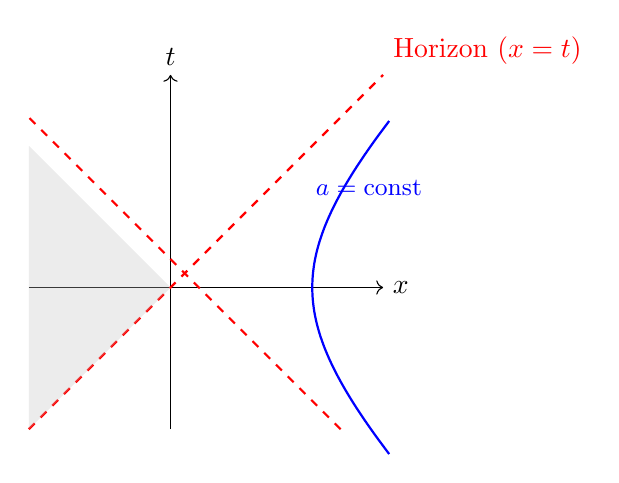
\begin{tikzpicture}[scale=1.8]
\draw[->] (-1,0) -- (1.5,0) node[right] {$x$};
\draw[->] (0,-1) -- (0,1.5) node[above] {$t$};
\draw[dashed, red, thick] (-1,-1) -- (1.5,1.5) node[above right] {Horizon ($x=t$)};
\draw[dashed, red, thick] (1.2,-1) -- (-1,1.2);
\draw[thick, blue, domain=-1:1, smooth, variable=\t] plot ({cosh(\t)}, {sinh(\t)});
\fill[lightgray, opacity=0.3] (-1,1) -- (0,0) -- (-1,-1) -- cycle;
\node[blue] at (1.4,0.7) {\small $a=\text{const}$};
\end{tikzpicture}
\caption{Spacetime diagram showing the Rindler horizon restricting vacuum mode access to an accelerating observer.}
\end{figure}
\section{The Geometric Peak: General Relativity}
\begin{equation}
G_{\mu\nu} + \Lambda g_{\mu\nu} = \frac{8\pi G}{c^4} T_{\mu\nu} \label{eq:efe}
\end{equation}
Varying $S_{\text{EH}} = \frac{1}{16\pi G} \int d^4x \sqrt{-g} R$ with respect to the inverse metric $g^{\mu\nu}$ using the metric determinant identity $\delta\sqrt{-g} = -\frac{1}{2}\sqrt{-g}g_{\mu\nu}\delta g^{\mu\nu}$:
\begin{equation}
\delta S_{\text{EH}} = \frac{1}{16\pi G} \int d^4x \sqrt{-g} \left( R_{\mu\nu} - \frac{1}{2}g_{\mu\nu}R \right) \delta g^{\mu\nu} = 0 \implies G_{\mu\nu} = R_{\mu\nu} - \frac{1}{2}g_{\mu\nu}R
\end{equation}
Introducing the Regge-Wheeler tortoise coordinate $r^* = r + r_s \ln \left| \frac{r}{r_s} - 1 \right|$ isolates path parameters:
\begin{equation}
V = \sqrt{\frac{r}{r_s} - 1} e^{\frac{r}{2r_s}} \cosh\left(\frac{ct}{2r_s}\right), \quad U = \sqrt{\frac{r}{r_s} - 1} e^{\frac{r}{2r_s}} \sinh\left(\frac{ct}{2r_s}\right)
\end{equation}
Executing standard substitution eliminates the singular denominator profile, revealing the fully regularized spacetime metric:
\begin{equation}
ds^2 = -\frac{32G^3M^3}{c^6 r} e^{-\frac{r}{r_s}} (dV^2 - dU^2) + r^2(d\theta^2 + \sin^2\theta , d\phi^2)
\end{equation}
Near the event horizon, proper spatial metrics mimic accelerating Rindler configurations governed by the black hole surface gravity $\kappa$:
\begin{equation}
|\beta_{\omega}|^2 = e^{-\frac{2\pi\omega}{\kappa}} |\alpha_{\omega}|^2 \implies \langle 0_K | \hat{N}_\omega | 0_K \rangle = \frac{1}{e^{\frac{2\pi\omega}{\kappa}} - 1} = \frac{1}{e^{\frac{8\pi GM\omega}{c^3}} - 1}
\end{equation}
Equating this result directly to a standard thermodynamic thermal profile yields the exact Hawking Temperature:
\begin{equation}
T_H = \frac{\hbar \kappa}{2\pi c k_B} = \frac{\hbar c^3}{8\pi G k_B M}
\end{equation}
\section{Quantum Field Theory in Curved Spacetime}
Before evaluating the thermodynamic properties of horizons, we must formalize the behavior of fields when a globally defined, unique Minkowski time parameter is absent. We consider a real scalar field $\Phi$ satisfying the covariant Klein-Gordon equation on a curved pseudo-Riemannian manifold $(\mathcal{M}, g)$:
\begin{equation}
\left( \square - m^2 - \xi R \right) \Phi = 0
\end{equation}
where $\square = g^{\mu\nu}\nabla_\mu\nabla_\nu$ represents the Laplace-Beltrami operator, and $\xi$ captures the non-minimal coupling to the scalar curvature $R$. We expand the field operator $\hat{\Phi}$ using a complete set of orthonormal basis modes $u_i$:
\begin{equation}
\hat{\Phi} = \sum_i \left( \hat{a}_i u_i + \hat{a}_i^{\dagger} u_i^* \right)
\end{equation}
If the spacetime admits a non-trivial gravitational collapse or features an acceleration horizon, an alternative, equally valid observer can establish a separate coordinate framework with basis modes $v_j$, yielding:
\begin{equation}
\hat{\Phi} = \sum_j \left( \hat{b}_j v_j + \hat{b}_j^{\dagger} v_j^* \right)
\end{equation}
Because the definition of a particle state relies entirely on the choice of positive-frequency modes, the creation and annihilation operators of the two observers mix dynamically via the Bogoliubov relationship: $\hat{b}j = \sum_i (\alpha{ji}\hat{a}i - \beta{ji}^*\hat{a}_i^{\dagger})$. This explains why a state perceived as an empty vacuum $|0\rangle$ by an inertial observer can be filled with a thermal flux when measured by a non-inertial observer.
\section{The Ultimate Unifier: Lagrangian Field Theory}
Modern field theories define configurations using a scalar density called the Lagrangian ($\mathcal{L}$). Extremizing the Action path integral functional $S = \int \mathcal{L} , d^4x$ yields the covariant Euler-Lagrange equations:
\begin{equation}
\partial_\mu \left( \frac{\partial \mathcal{L}}{\partial(\partial_\mu \phi)} \right) - \frac{\partial \mathcal{L}}{\partial \phi} = 0
\end{equation}
Given a particle baseline setup defined by $\mathcal{L} = \frac{1}{2}m\dot{x}^2 - V(x)$, evaluating coordinates yields:
\begin{equation}
\frac{\partial \mathcal{L}}{\partial \dot{x}} = m\dot{x}, \quad \frac{d}{dt}\left(\frac{\partial \mathcal{L}}{\partial \dot{x}}\right) = m\ddot{x}, \quad \frac{\partial \mathcal{L}}{\partial x} = -\frac{\partial V}{\partial x} = F \implies F = ma
\end{equation}
When expanding local symmetries to gauge fields, minimal coupling transforms the structural dynamics:
\begin{equation}
\mathcal{L}{\text{Maxwell}} = -\frac{1}{4}F{\mu\nu}F^{\mu\nu} - \mu_0 J^\mu A_\mu, \quad \mathcal{L}{\text{QED}} = \bar{\psi}(i\gamma^\mu D{\mu} - m)\psi - \frac{1}{4}F_{\mu\nu}F^{\mu\nu}
\end{equation}
To evaluate parameter behavior across shifting energy regimes, we formulate the Callan-Symanzik relationship:
\begin{equation}
\left[ \mu \frac{\partial}{\partial \mu} + \beta(g) \frac{\partial}{\partial g} + n \gamma_{\phi} \right] G^{(n)}(x_1, \dots, x_n; \mu, g) = 0
\end{equation}
\begin{figure}[h!]
\centering
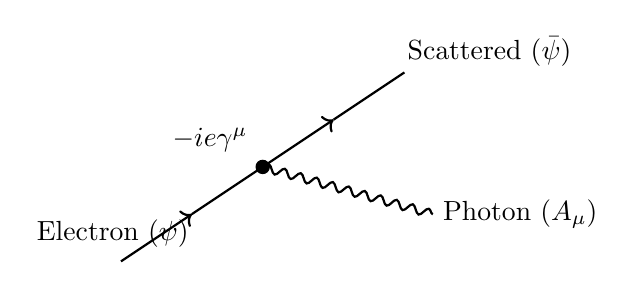
\begin{tikzpicture}[scale=1.2]
\coordinate (v);
\draw[thick, ->] (-1.5,-1) -- (-0.75,-0.5);
\draw[thick] (-0.75,-0.5) -- (v) node[pos=0.1, below left] {Electron ($\psi$)};
\draw[thick, ->] (v) -- (0.75,0.5);
\draw[thick] (0.75,0.5) -- (1.5,1) node[pos=0.9, above right] {Scattered ($\bar{\psi}$)};
\draw[thick, decorate, decoration={snake, amplitude=1.5pt, segment length=6pt}] (v) -- (1.8,-0.5) node[right] {Photon ($A_\mu$)};
\filldraw[black] (v) circle (2pt) node[above left=0.1cm] {$-ie\gamma^\mu$};
\end{tikzpicture}
\caption{Feynman diagram visualizing the QED vertex interaction dictated by the minimal coupling term.}
\end{figure}
\section{Foundations of Quantum Mechanics}
The temporal evolution and canonical geometry of non-commuting variables are structured as:
\begin{equation}
i\hbar \frac{\partial}{\partial t}|\psi(t)\rangle = \hat{H}|\psi(t)\rangle, \quad [\hat{x}, \hat{p}] = i\hbar
\end{equation}
When these canonical quantization rules are fully expanded into General Relativity metrics, the explicit background time parameter disappears completely. This results in the timeless Wheeler-DeWitt state equation:
\begin{equation}
\hat{H}_{\text{Wheeler-DeWitt}}|\Psi\rangle = 0
\end{equation}
\section{Topological Solitons, Instantons and Anomalies}
The Chern-Simons action, the QCD $\theta$-vacuum term, and the axial current anomaly are formulated as:
\begin{equation}
S_{\text{CS}} = \frac{k}{4\pi} \int \text{Tr}\left(A \wedge dA - \frac{2}{3}i A \wedge A \wedge A\right), \quad \partial_\mu j^\mu_5 = \frac{e^2}{16\pi^2} F_{\mu\nu}\tilde{F}^{\mu\nu}
\end{equation}
\section{Supersymmetry and Supergravity (SUGRA)}
Supersymmetry transforms spacetime classifications by mapping bosonic degrees of freedom directly to fermionic ones, forming matching Wess-Zumino interaction mechanics:
\begin{equation}
{Q_\alpha, \bar{Q}{\dot{\beta}}} = 2\sigma^\mu{\alpha\dot{\beta}} P_mu, \quad \mathcal{L}{\text{WZ}} = \partial{\mu} \phi^\dagger \partial^\mu \phi + i\bar{\psi}\bar{\sigma}^\mu \partial_\mu \psi + \left|\frac{\partial W}{\partial \phi}\right|^2
\end{equation}
\section{String Theory and Conformal Field Theory (CFT)}
Replacing 0D point particles with 1D oscillating strings maps physical tracks onto a 2D worldsheet embedding profile. The continuous geometric mechanics are governed by the Polyakov action and the corresponding Virasoro algebra parameters:
\begin{equation}
S_P = -\frac{T}{2} \int d^2\sigma \sqrt{-\gamma}\gamma^{\alpha\beta}\partial_\alpha X^\mu \partial_\beta X^\nu g_{\mu\nu}(X), \quad [L_m, L_n] = (m-n)L_{m+n} + \frac{c}{12}m(m^2-1)\delta_{m+n,0}
\end{equation}
\section{The Gauge/Gravity Duality (AdS/CFT Correspondence)}
The holographic principle states that quantum gravity configurations within an Anti-de Sitter ($AdS$) bulk space map exactly onto a non-gravitational Conformal Field Theory ($CFT$) residing on the boundary~\cite{Maldacena1998}. The Ryu-Takayanagi relation elegantly equates quantum entanglement entropy directly to a minimal geometric area:
\begin{equation}
Z_{\text{Gravity}}[\phi_0] = \left\langle \exp\left(\int \mathcal{O}\phi_0\right) \right\rangle_{\text{CFT}}, \quad R^4 = 4\pi g_s N \ell_s^4, \quad S_A = \frac{\text{Area}(\gamma_A)}{4G_N}
\end{equation}
Let subregion $A$ be a one-dimensional line interval on the boundary ($z \to 0$) stretching from $x = -l/2$ to $x = l/2$. The surface area integral for a profile path $z(x)$ entering the bulk is given by:
\begin{equation}
\text{Area}(\gamma_A) = \int_{-l/2}^{l/2} \frac{R}{z} \sqrt{1 + \left(\frac{dz}{dx}\right)^2} dx
\end{equation}
Extremizing this functional via the Euler-Lagrange equations yields a semicircular path profile, $x^2 + z^2 = (l/2)^2$, defining the radial depth explicitly as $z = \sqrt{(l/2)^2 - x^2}$. Differentiating this profile gives $\frac{dz}{dx} = -\frac{x}{\sqrt{(l/2)^2 - x^2}}$, causing the arc-length parameter to collapse cleanly. Substituting these back into the area functional yields the geometrically accurate integrand:
\begin{equation}
\begin{aligned}
\text{Area}(\gamma_A) &= 2 \int_0^{\sqrt{(l/2)^2 - \epsilon^2}} \frac{R}{\sqrt{(l/2)^2 - x^2}} \cdot \frac{l/2}{\sqrt{(l/2)^2 - x^2}} , dx \
&= 2 \int_0^{\sqrt{(l/2)^2 - \epsilon^2}} \frac{R(l/2)}{(l/2)^2 - x^2} , dx
\end{aligned}
\end{equation}
Evaluating this via partial fractions up to the ultraviolet cutoff regulator scale $\epsilon$ yields:
\begin{equation}
\text{Area}(\gamma_A) = 2 \left[ \frac{R}{2} \ln\left| \frac{\frac{l}{2} + x}{\frac{l}{2} - x} \right| \right]_0^{\sqrt{(l/2)^2 - \epsilon^2}} = 2R \ln\left( \frac{\frac{l}{2} + \sqrt{(\frac{l}{2})^2 - \epsilon^2}}{\epsilon} \right) \approx 2R \ln\left( \frac{l}{\epsilon} \right)
\end{equation}
Dividing by the gravitational constant $4G_N$, we arrive at the exact conformal field entanglement entropy:
\begin{equation}
S_A = \frac{c}{3} \ln\left( \frac{l}{\epsilon} \right)
\end{equation}
\begin{figure}[h!]
\centering
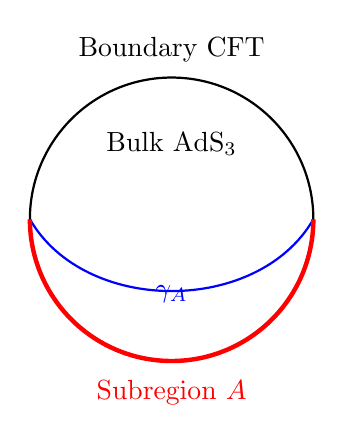
\begin{tikzpicture}[scale=1.2]
\draw[thick] (0,0) circle (1.5);
\draw[blue, thick] (-1.5,0) to[out=-60,in=-120] (1.5,0);
\draw[red, ultra thick] (-1.5,0) arc (180:360:1.5);
\node at (0,0.8) {Bulk $\text{AdS}_3$};
\node[blue, below] at (0,-0.6) {$\gamma_A$};
\node[red, below] at (0,-1.6) {Subregion $A$};
\node at (0,1.8) {Boundary CFT};
\end{tikzpicture}
\caption{Geometric visualization of the Ryu-Takayanagi minimal area surface extending into the bulk interior.}
\end{figure}
\section{Statistical Mechanics and Thermodynamics}
When tracking discrete microstates becomes unfeasible, statistical systems treat phase space geometry distributions through the canonical partition function $Z$ and the statistical Boltzmann entropy definition:
\begin{equation}
Z = \sum_i e^{-\beta E_i}, \quad \beta = \frac{1}{k_B T}, \quad S = k_B \ln \Omega
\end{equation}
\section{The Particle Frontier: The Higgs \& Standard Model Lagrangian}
Mass generation within the Standard Model is driven by the mechanisms of spontaneous symmetry breaking when a complex scalar field develops a non-zero vacuum expectation value ($vev$) within the Higgs scalar potential parameters, as detailed by Peter Higgs~\cite{Higgs1964}. To frame this globally, we synthesize the localized gauge fields into the complete Standard Model Lagrangian layout expression, split cleanly across multiple lines to fit the page geometry:
\begin{equation}
\begin{aligned}
\mathcal{L}_{\text{SM}} = & -\frac{1}{4}G_{\mu\nu}^a G^{\mu\nu a} - \frac{1}{4}W_{\mu\nu}^a W^{\mu\nu a} - \frac{1}{4}B_{\mu\nu}B^{\mu\nu} \\
& + \bar{\psi}_i i\gamma^\mu D_\mu \psi_i + |D_\mu \phi|^2 \\
& - (\mu^2 \phi^\dagger \phi + \lambda(\phi^\dagger \phi)^2) \\
& - (y_{ij}\bar{\psi}_i \phi \psi_j + \text{h.c.})
\end{aligned}
\end{equation}

\section{Early Universe Inflation and Cosmological Perturbations}
To explain the global flatness and homogeneity of the cosmos described in the subsequent section, we introduce a phase of accelerated geometric expansion driven by a scalar inflaton field $\phi$. The dynamics are governed by the action of a minimally coupled field interacting with a Higgs-like potential $V(\phi)$:
\begin{equation}
S_{\text{inf}} = \int d^4x \sqrt{-g} \left( -\frac{1}{2} g^{\mu\nu} \partial_\mu \phi \partial_\nu \phi - V(\phi) \right)
\end{equation}
Enforcing the homogeneous FLRW background metric reduces the equations of motion to the standard cosmic slow-roll evolution: $\ddot{\phi} + 3H\dot{\phi} + V'(\phi) = 0$. During this epoch, microscopic quantum fluctuations $\delta\phi$ are stretched rapidly across the expanding horizon layout. The power spectrum of these frozen geometric curvature perturbations is formulated as:
\begin{equation}
\mathcal{P}{\mathcal{R}}(k) = \frac{H^2}{2\pi \dot{\phi}} \biggr\vert{k=aH}
\end{equation}
These amplified fluctuations act as the primordial seeds of cosmic structure, illustrating how quantum fields can be stretched geometrically to construct the large-scale architecture of our universe.
\section{Cosmology: The Geometry of the Entire Cosmos}
Enforcing spatial homogeneity and isotropy across large-scale celestial landscapes isolates the metric scaling behavior of our expanding universe via the FLRW metric profile and the dynamic Friedmann field equations:
\begin{equation}
ds^2 = -c^2dt^2 + a(t)^2 \left[ \frac{dr^2}{1 - kr^2} + r^2(d\theta^2 + \sin^2\theta \, d\phi^2) \right], \quad \left(\frac{\dot{a}}{a}\right)^2 = \frac{8\pi G}{3}\rho - \frac{kc^2}{a^2} + \frac{\Lambda c^2}{3}
\end{equation}
\newpage
\addcontentsline{toc}{section}{References}
\nocite{*}
\printbibliography
\end{document}
